\section{KHÁI NIỆM VECTƠ}
\subsection{TÓM TẮT LÝ THUYẾT}
\subsubsection{Khái niệm vectơ}
Cho đoạn thẳng $AB$ . Nếu chọn điểm $A$  làm điểm đầu, điểm  $B$ làm điểm cuối thì đoạn thẳng $AB$  có hướng từ $A$  đến $B$ . Khi đó ta nói  $AB$ là một \indamm{đoạn thẳng có hướng}.	
		\begin{itemize}
		\item[\iconMT] \indam{ Định nghĩa: }
		\begin{itemize}
			\item  Vectơ là một đoạn thẳng có hướng, nghĩa là trong hai điểm mút của đoạn thẳng đã chỉ rõ điểm đầu, điểm cuối.
			\item  Độ dài vectơ là khoảng cách giữa điểm đầu và điểm cuối của vectơ đó.
		\end{itemize}
		\item[\iconMT]\indam{ Chú ý:}
		\immini{
			\begin{itemize}
			\item Nếu chỉ rõ điểm đầu là $A$ và điểm cuối là $B$, ta có "vectơ $AB$", kí hiệu $\vec{AB}$. Nếu không cần chỉ rõ điểm đầu và điểm cuối, ta dùng các chữ cái thường để kí hiệu. Ví dụ $\vec{a}, \vec{b}, \vec{x},...$
			\item  Độ dài $\vec{a}$, kí hiệu $|\vec{a}|$; Độ dài $\vec{AB}$, kí hiệu $|\vec{AB}|$ và hiển nhiên $|\vec{AB}|=AB$.
			\end{itemize}	}{
	\hspace{2cm}
		\begin{tikzpicture}[smooth,samples=300,scale=0.8,>=stealth,font=\footnotesize]
		\tkzDefPoints{0/0/A,3/1/B}
		\draw[->] (0,0)--(3,1);
		\draw[->] (1,-1)--(4,-1);
		\tkzDrawPoints[size=2,fill=black](A,B)
		\node[below] at (3,-1) {$\vec{x}$};
		\tkzLabelPoints[below](A)
		\tkzLabelPoints[below right](B)
		\end{tikzpicture}}
	\end{itemize}

\subsubsection{Vectơ cùng phương, cùng hướng}
Đường thẳng đi qua điểm đầu và điểm cuối của vectơ gọi là giá của vectơ đó.
	\begin{itemize}
		\item[\iconMT] Hai vectơ cùng phương nếu giá của chúng song song hoặc trùng nhau.	
		\item[\iconMT] Khi hai vectơ cùng phương, chúng có thể cùng hướng hoặc ngược hướng.
	\end{itemize}
\subsubsection{Vectơ bằng nhau}
Hai vec tơ $\vec{a}$ và $\vec{b}$ được gọi là bằng nhau, kí hiệu $\vec{a}=\vec{b}$ nếu chúng có cùng hướng và cùng độ dài.
\subsubsection{Vectơ-không}
	\begin{itemize}
		\item[\iconMT] \indam{Định nghĩa: }Là vectơ có điểm đầu và điểm cuối trùng nhau. 
		\begin{itemize}
			\item Kí hiệu $\vec{0}$, nghĩa là $\vec{0}=\vec{AA}=\vec{BB}$...;
			\item Độ dài vectơ-không bằng $0$, nghĩa là $\bigg|\vec{0}\bigg|=0$.
		\end{itemize}

		\item[\iconMT]  \indam{Qui ước: }Vec tơ-không cùng phương và cùng hướng với mọi véc tơ.
	\end{itemize}
\subsection{RÈN LUYỆN KĨ NĂNG GIẢI TOÁN}

\begin{dang}{Xác định vectơ, vectơ cùng phương, vectơ cùng hướng, vectơ ngược hướng}
\end{dang}

\begin{vd}
	\immini{Cho tam giác $ABC$. Hãy kể tên các vectơ (khác $\vec{0}$) có điểm đầu và điểm cuối là các đỉnh $A$, $B$, $C$.}{
		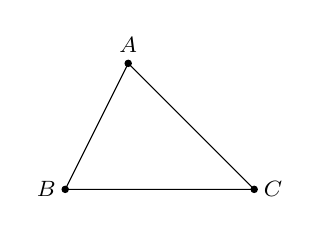
\begin{tikzpicture}[smooth,font=\footnotesize,scale=0.8]
		\path
		(0,0) coordinate (B)
		(3,0) coordinate (C)
		(1,2) coordinate (A);
		\draw (A)--(B)--(C)--(A);
		\foreach \x/\g in {A/90,B/180,C/0} \draw [fill=black] (\x) circle (.05) + (\g:.3) node{$\x$};
\end{tikzpicture}}
\loigiai{
Các vec tơ có thể là $\vec{AB}$, $\vec{AC}$, $\vec{BC}$, $\vec{BA}$, $\vec{CA}$, $\vec{CB}$.}
\end{vd} \dongcham{1}


\begin{vd}
	\immini{Cho hình bình hành $ABCD$ tâm $O$. Trên hình bên, 
	\begin{tasks}(1)
		\task Kể tên 2 vectơ cùng phương với véc tơ $\vec{OA}$.
		\task Kể tên vectơ cùng hướng, ngược hướng với véc tơ $\vec{OB}$.
	\end{tasks}
}{
		\begin{tikzpicture}[smooth,font=\footnotesize,scale=0.8]
			\path
			(0,0) coordinate (A)
			(1,2) coordinate (B)
			(4,2) coordinate (C)
			(3,0) coordinate (D);
			\coordinate (O) at ($(C)!0.5!(A)$);
			\draw (A)--(B)--(C)--(D)--cycle (A)--(C) (B)--(D);
			\foreach \x/\g in {A/-90,B/90,C/90,D/-90,O/90} \draw [fill=black] (\x) circle (.05) + (\g:.3) node{$\x$};
	\end{tikzpicture}}
\loigiai{
\begin{enumerate}[a)]
	\item Hai vec tơ cùng phương với $\vec{OA}$ là $\vec{AC}$, $\vec{OC}$ hoặc $\vec{CA}$, $\vec{OA}$,...
	\item Vec tơ cùng hướng với $\vec{OB}$ là $\vec{DB}$; hướng với $\vec{OB}$ là $\vec{BO}$ và $\vec{BD}$.
\end{enumerate}}
\end{vd} \dongcham{1}

\begin{vd}
	\immini{
		Cho ba điểm $A$, $B$, $C$ thẳng hàng, $B$ nằm giữa $A$ và $C$. Chỉ ra ba cặp vectơ khác $\overrightarrow{0}$ có điểm đầu và điểm cuối trong các điểm $A$, $B$, $C$ thoả mãn:
		\begin{enumEX}[a)]{2}
			\item Cặp vectơ đó cùng hướng.
			\item Cặp vectơ đó ngược hướng.
		\end{enumEX}
	}{
		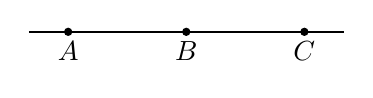
\begin{tikzpicture}[>=stealth, scale=1]
			\draw[thick] (0,0) -- (4,0);
			\fill (0.5,0) circle (1.5pt) node[below] {$A$};
			\fill (2,0) circle (1.5pt) node[below] {$B$};
			\fill (3.5,0) circle (1.5pt) node[below] {$C$};
		\end{tikzpicture}
	}
	\loigiai{
		Vì ba điểm $A, B, C$ thẳng hàng và $B$ nằm giữa $A$ và $C$ nên ta có hai nhóm vectơ (khác $\overrightarrow{0}$) cùng hướng với nhau:
		\begin{itemize}
			\item \textbf{Nhóm 1} (hướng từ $A$ đến $C$): $\overrightarrow{AB}, \overrightarrow{BC}, \overrightarrow{AC}$.
			\item \textbf{Nhóm 2} (hướng từ $C$ đến $A$): $\overrightarrow{CB}, \overrightarrow{BA}, \overrightarrow{CA}$.
		\end{itemize}
		Dựa vào phân tích trên, ta có thể dễ dàng chỉ ra:
		\begin{enumerate}
			\item[a)] Ba cặp vectơ cùng hướng (chọn ngẫu nhiên 2 vectơ cùng thuộc một nhóm). Ví dụ:
			$$ \left(\overrightarrow{AB}, \overrightarrow{AC}\right);\quad \left(\overrightarrow{AB}, \overrightarrow{BC}\right);\quad \left(\overrightarrow{BA}, \overrightarrow{CA}\right). $$
			\item[b)] Ba cặp vectơ ngược hướng (chọn 1 vectơ thuộc nhóm 1 và 1 vectơ thuộc nhóm 2). Ví dụ:
			$$ \left(\overrightarrow{AB}, \overrightarrow{BA}\right);\quad \left(\overrightarrow{AB}, \overrightarrow{CB}\right);\quad \left(\overrightarrow{AC}, \overrightarrow{CA}\right). $$
		\end{enumerate}
	}
\end{vd}
\dongcham{1}
\begin{dang}{Vectơ bằng nhau}
\end{dang}

\begin{vd}
	\immini{Cho tam giác $ABC$. Các điểm $M$, $N$ và $K$ lần lượt là trung điểm của $AB$, $AC$ và $BC$.
		\begin{tasks}(1)
			\task Tìm các vectơ bằng với $\vec{AM}$.
			\task Tìm các vectơ bằng với $\vec{KN}$.
	\end{tasks}}{\hspace{1cm}
		\begin{tikzpicture}[scale=0.8, line join=round, line cap=round]
		\tkzDefPoints{0/0/A,1/2/B,4/0/C}
		\coordinate (M) at ($(A)!0.5!(B)$);
		\coordinate (N) at ($(C)!0.5!(A)$);
		\coordinate (K) at ($(B)!0.5!(C)$);
		\tkzDrawSegments(A,B B,C C,A M,N N,K M,K)
		\tkzDrawPoints[size=2,fill=black](A,B,C,M,N,K)
		\tkzLabelPoints[below, font=\footnotesize](A,N,C)
		\tkzLabelPoints[above, font=\footnotesize](B)
		\tkzLabelPoints[above left, font=\footnotesize](M)
		\tkzLabelPoints[above right, font=\footnotesize](K)
		\end{tikzpicture}}
	\loigiai{
	\begin{enumerate}
		\item[a)] Các vectơ bằng với $\overrightarrow{AM}$ (cùng hướng và cùng độ dài với $\overrightarrow{AM}$) là: $\overrightarrow{MB}$ và $\overrightarrow{NK}$.
		\item[b)] Các vectơ bằng với $\overrightarrow{KN}$ (cùng hướng và cùng độ dài với $\overrightarrow{KN}$) là: $\overrightarrow{MA}$ và $\overrightarrow{BM}$.
\end{enumerate}}
\end{vd} \dongcham{3}

\begin{vd}
	\immini{Cho lục giác đều $ABCDEF$ tâm $O$.
		\begin{tasks}(1)
			\task Tìm các vectơ bằng với $\vec{EF}$.
			\task Tìm các vectơ bằng với $\vec{OB}$.
	\end{tasks}}{\hspace{1cm}
		\begin{tikzpicture}[scale=0.7]
		\tkzDefPoint(0,0){O}
		\tkzDefPoint(2,0){E}
		\tkzDefPointBy[rotation = center O angle 60](E) \tkzGetPoint{F}
		\tkzDefPointBy[rotation = center O angle 120](E) \tkzGetPoint{A}
		\tkzDefPointBy[rotation = center O angle 180](E) \tkzGetPoint{B}
		\tkzDefPointBy[rotation = center O angle 240](E) \tkzGetPoint{C}
		\tkzDefPointBy[rotation = center O angle 300](E) \tkzGetPoint{D}
		\tkzDrawPoints[size=2,fill=black](A,B,C,D,E,F,O)
		\tkzDrawSegments(A,B B,C C,D D,E E,F F,A)
		\draw (A) node[above] {$A$} (B) node[left] {$B$} (C) node[below] {$C$} (D) node[below] {$D$} (E) node[right] {$E$} (F) node[above] {$F$} (O) node[below left] {$O$};
		\end{tikzpicture}}
	\loigiai{
	\begin{enumerate}
		\item[a)] Các vectơ bằng với $\overrightarrow{EF}$ (cùng hướng và cùng độ dài với $\overrightarrow{EF}$) là: $\overrightarrow{DO}, \overrightarrow{OA}$ và $\overrightarrow{CB}$.
		\item[b)] Các vectơ bằng với $\overrightarrow{OB}$ (cùng hướng và cùng độ dài với $\overrightarrow{OB}$) là: $\overrightarrow{DC}, \overrightarrow{EO}$ và $\overrightarrow{FA}$.
\end{enumerate}}
\end{vd} \dongcham{1}

\begin{vd}
	\immini{Cho tam giác $ABC$ có trọng tâm $G$. Gọi $I$ là trung điểm của $BC$. Dựng điểm $B'$ thỏa $\vec{B'B}=\vec{AG}$.
	\begin{tasks}(1)
		\task Chứng minh $\vec{BI}=\vec{IC}$
		\task Gọi $K$ là trung điểm của $BB'$. Chứng minh rằng $\vec{BK}=\vec{IG}$.
	\end{tasks}
}{
	\hspace{1cm}
	\begin{tikzpicture}[scale=1, line join=round, line cap=round]
	\tkzDefPoints{0/0/B,4/0/C, 1/2/A}
	\coordinate (I) at ($(C)!0.5!(B)$);
	\tkzCentroid(A,B,C)\tkzGetPoint{G}
	\coordinate (B') at ($(A)+(B)-(G)$);
	\tkzDrawSegments(A,B B,C C,A B',B A,I)
	\tkzDrawPoints[size=2,fill=black](A,B,C,I,G,B')
	\tkzLabelPoints[below,font=\footnotesize](B,C,I)
	\tkzLabelPoints[above,font=\footnotesize](A,B')
	\tkzLabelPoints[below left,font=\footnotesize](G)
	\end{tikzpicture}}
\loigiai{
\begin{enumerate}
	\item[a)] Vì $G$ là trọng tâm của tam giác $ABC$ nên ta có đẳng thức vectơ:
	$$ \overrightarrow{GA} + \overrightarrow{GB} + \overrightarrow{GC} = \vec{0} \Leftrightarrow -\overrightarrow{AG} + \overrightarrow{GB} + \overrightarrow{GC} = \vec{0} \Leftrightarrow \overrightarrow{AG} = \overrightarrow{GB} + \overrightarrow{GC} $$
	Theo quy tắc ba điểm, ta chèn điểm $B$ vào vectơ $\overrightarrow{B'G}$:
	$$ \overrightarrow{B'G} = \overrightarrow{B'B} + \overrightarrow{BG} = \overrightarrow{B'B} - \overrightarrow{GB} $$
	Mà theo giả thiết $\overrightarrow{B'B} = \overrightarrow{AG}$, thay vào ta được:
	$$ \overrightarrow{B'G} = \overrightarrow{AG} - \overrightarrow{GB} = (\overrightarrow{GB} + \overrightarrow{GC}) - \overrightarrow{GB} = \overrightarrow{GC} \text{ (điều phải chứng minh).} $$
	
	\item[b)] Vì $K$ là trung điểm của đoạn thẳng $BB'$ nên:
	$$ \overrightarrow{BK} = \dfrac{1}{2}\overrightarrow{BB'} = -\dfrac{1}{2}\overrightarrow{B'B} = -\dfrac{1}{2}\overrightarrow{AG} $$
	Mặt khác, $G$ là trọng tâm tam giác $ABC$ và $I$ là trung điểm của $BC$ nên $A, G, I$ thẳng hàng, $G$ nằm giữa $A$ và $I$, đồng thời $AG = 2GI$.
	Viết dưới dạng vectơ, ta có: $\overrightarrow{AG} = 2\overrightarrow{GI} = -2\overrightarrow{IG}$.\\
	Thay đẳng thức này vào biểu thức của $\overrightarrow{BK}$, ta thu được:
	$$ \overrightarrow{BK} = -\dfrac{1}{2}(-2\overrightarrow{IG}) = \overrightarrow{IG} \text{ (điều phải chứng minh).} $$
\end{enumerate}}
\end{vd} \dongcham{4}

\begin{dang}{Độ dài véc tơ}
	Độ dài $\vec{AB}$ là độ dài đoạn thẳng $AB$. Khi tính toán, ta có thể chú ý đến định lý Pitago và các tỉ số lượng giác của góc nhọn trong tam giác vuông.
\end{dang}

\begin{vd}
	\immini{Cho hình vuông $ABCD$ tâm $O$, cạnh bằng 2. 
		\begin{tasks}(1)
			\task Tính độ dài của các vec tơ $\vec{AB}$, $\vec{AC}$, $\vec{AO}$.
			\task Gọi $I$ là trung điểm của $BC$. Tính độ dài vec tơ $\vec{AI}$.
		\end{tasks}
	}{\hspace{1cm}
		\begin{tikzpicture}[smooth,font=\footnotesize,scale=1]
			\path
			(0,0) coordinate (A)
			(2,0) coordinate (B)
			(2,2) coordinate (C)
			(0,2) coordinate (D);
			\coordinate (O) at ($(B)!0.5!(D)$);
			\draw (A)--(B)--(C)--(D)--(A) (A)--(C) (B)--(D);
			\foreach \x/\g in {A/-90,B/-90,C/90,D/90,O/0} \draw [fill=black] (\x) circle (.05) + (\g:.3) node{$\x$};
	\end{tikzpicture}}
	\loigiai{
	\begin{enumerate}
		\item[a)] Ta có độ dài vectơ $\overrightarrow{AB}$ chính là độ dài đoạn thẳng $AB$. Do đó: $|\overrightarrow{AB}| = AB = 2$.\\
		Xét tam giác $ABC$ vuông tại $B$, áp dụng định lý Pythagore ta có:
		$$ AC = \sqrt{AB^2 + BC^2} = \sqrt{2^2 + 2^2} = \sqrt{8} = 2\sqrt{2}. $$
		Do đó, $|\overrightarrow{AC}| = AC = 2\sqrt{2}$.\\
		Vì $O$ là tâm hình vuông nên $O$ là trung điểm của đường chéo $AC$, suy ra:
		$$ AO = \dfrac{1}{2}AC = \dfrac{1}{2} \cdot 2\sqrt{2} = \sqrt{2}. $$
		Do đó, $|\overrightarrow{AO}| = AO = \sqrt{2}$.
		
		\item[b)] Vì $I$ là trung điểm của đoạn thẳng $BC$ nên $BI = \dfrac{1}{2}BC = \dfrac{1}{2} \cdot 2 = 1$.\\
		Xét tam giác $ABI$ vuông tại $B$, áp dụng định lý Pythagore ta có:
		$$ AI = \sqrt{AB^2 + BI^2} = \sqrt{2^2 + 1^2} = \sqrt{5}. $$
		Vậy độ dài vectơ $\overrightarrow{AI}$ là $|\overrightarrow{AI}| = AI = \sqrt{5}$.
	\end{enumerate}
}
\end{vd} \dongcham{3}

\begin{vd}
	Cho tam giác $ABC$ đều, cạnh bằng 3. Gọi $H$ là trung điểm của $BC$ và $G$ là trọng tâm tam giác $ABC$.
	\begin{tasks}(2)
		\task Hãy tính độ lớn của vectơ $\vec{AH}$
		\task Hãy tính độ lớn của vectơ $\vec{AG}$
	\end{tasks}
	\loigiai{
	\begin{enumerate}
		\item[a)] Vì tam giác $ABC$ là tam giác đều cạnh bằng $3$ và $H$ là trung điểm của $BC$ nên $AH$ là đường trung tuyến, đồng thời là đường cao của tam giác.\\
		Ta có công thức tính độ dài đường cao của tam giác đều cạnh $a$ là $h = \dfrac{a\sqrt{3}}{2}$.\\
		Áp dụng vào tam giác $ABC$ có cạnh $a=3$, ta được: $AH = \dfrac{3\sqrt{3}}{2}$.\\
		Vậy độ lớn của vectơ $\overrightarrow{AH}$ là $|\overrightarrow{AH}| = AH = \dfrac{3\sqrt{3}}{2}$.
		
		\item[b)] Vì $G$ là trọng tâm của tam giác $ABC$ và $AH$ là đường trung tuyến nên ta có hệ thức về độ dài:
		$$ AG = \dfrac{2}{3}AH = \dfrac{2}{3} \cdot \dfrac{3\sqrt{3}}{2} = \sqrt{3}. $$
		Vậy độ lớn của vectơ $\overrightarrow{AG}$ là $|\overrightarrow{AG}| = AG = \sqrt{3}$.
	\end{enumerate}
}
\end{vd} \dongcham{3}